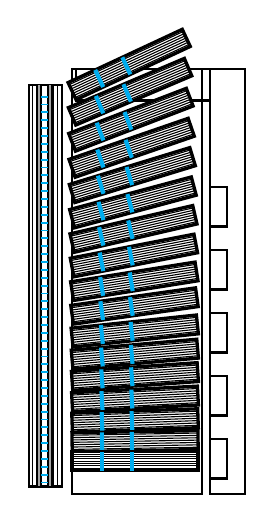
\begin{tikzpicture}[x=1cm, y=1cm]

% ----------------------------------------------------------
% COORDINATE SYSTEM (matching full diagram):
%   Preshower ~x=0.00..0.40
%   EE        ~x=0.55..2.20
%   Support   ~x=2.30..2.75
%   y range   ~0.0..5.5
% ----------------------------------------------------------

% ==========================================================
% 1. PRESHOWER (ES)
%    Thin vertical box with:
%    - outer frame (thick)
%    - several internal vertical dividers (thin/medium)
%    - dense cyan horizontal lines between innermost layers
% ==========================================================

% Outer frame
\fill[white]  (0.00, 0.20) rectangle (0.42, 5.30);
\draw[thick]  (0.00, 0.20) rectangle (0.42, 5.30);

% Outer thin gap lines
\draw[thin]   (0.05, 0.20) -- (0.05, 5.30);
\draw[thin]   (0.37, 0.20) -- (0.37, 5.30);

% Two absorber/sensor layers (thicker bands)
\fill[gray!70] (0.10, 0.20) rectangle (0.16, 5.30);
\draw[thick]   (0.10, 0.20) -- (0.10, 5.30);
\draw[thick]   (0.16, 0.20) -- (0.16, 5.30);

\fill[gray!70] (0.24, 0.20) rectangle (0.30, 5.30);
\draw[thick]   (0.24, 0.20) -- (0.24, 5.30);
\draw[thick]   (0.30, 0.20) -- (0.30, 5.30);

% Dense cyan horizontal strip lines between the two layers
\foreach \y in {0.25,0.35,...,5.25} {
  \draw[cyan, line width=0.7pt] (0.16, \y) -- (0.24, \y);
}

% ==========================================================
% 2. OUTER SUPPORT STRUCTURE (right side)
%    Large vertical plate + top horizontal bar
%    5 rectangular notches cut into left face
% ==========================================================

% Top horizontal connecting bar
\fill[white]  (0.60, 5.10) rectangle (2.30, 5.50);
\draw[thick]  (0.60, 5.10) rectangle (2.30, 5.50);

% Main vertical support plate
\fill[white]  (2.30, 0.10) rectangle (2.75, 5.50);
\draw[thick]  (2.30, 0.10) rectangle (2.75, 5.50);

% 5 rectangular notches on left face of support
\foreach \yn/\yh in {
  0.30/0.80,
  1.10/1.60,
  1.90/2.40,
  2.70/3.20,
  3.50/4.00
}{
  \fill[white]  (2.30, \yn) rectangle (2.52, \yh);
  \draw[thick]  (2.30, \yn) rectangle (2.52, \yh);
}

% ==========================================================
% 3. ENDCAP ECAL (EE)
%    ~20 supercrystal rows, each a rotated rectangle
%    - white fill, thick outer border
%    - ~8 internal thin horizontal lines (crystal separators)
%    - 2 vertical cyan lines at fixed fractions of width
%    Tilt: top rows ~22 deg, bottom rows ~3 deg (pointing to IP)
%    The left edge of each row is at ~x=0.55
%    Width of each row ~1.60 cm, height ~0.27 cm
%    The two cyan lines are at x=0.38 and x=0.76 of the row width
% ==========================================================

% Outer envelope of EE (thin line around all supercrystals)
% Computed from min/max of rotated rectangles — approximate:
\draw[thick] (0.55, 0.10) -- (2.20, 0.10) -- (2.20, 5.50) -- (0.55, 5.50) -- cycle;

% Parameters for EE rows
% Format: yCenter, angle (degrees, positive = CCW from x-axis)
% Angle is atan2(yC, zC) where zC~11 in real coords; we rescale visually.
% In image: top ~25 deg tilt, bottom ~2 deg tilt, ~20 rows.
\def\gW{1.60}  % crystal row length (local x)
\def\gH{0.24}  % crystal row height (local y)
\def\cxA{0.38} % cyan line 1 x position (local)
\def\cxB{0.76} % cyan line 2 x position (local)
\def\nLines{7}  % number of internal horiz separators

\foreach \rowI/\yC/\ang in {
   1/5.22/25,
   2/4.90/23,
   3/4.57/21,
   4/4.24/19,
   5/3.92/17,
   6/3.60/15,
   7/3.29/13,
   8/2.98/11,
   9/2.68/ 9,
  10/2.38/ 8,
  11/2.09/ 6,
  12/1.81/ 5,
  13/1.54/ 4,
  14/1.27/ 3,
  15/1.01/ 2,
  16/0.76/ 1,
  17/0.52/ 0
}{
  \begin{scope}[shift={(0.55,\yC)}, rotate=\ang]
    % White fill
    \fill[white] (0, {-\gH/2}) rectangle (\gW, {\gH/2});
    % Thick outer border
    \draw[line width=1.2pt, black] (0, {-\gH/2}) rectangle (\gW, {\gH/2});
    % Internal horizontal crystal separators (thin)
    \pgfmathsetmacro{\step}{\gH/(\nLines+1)}
    \foreach \k in {1,...,\nLines}{
      \pgfmathsetmacro{\yk}{-\gH/2 + \k*\step}
      \draw[thin, black] (0, \yk) -- (\gW, \yk);
    }
    % Two vertical cyan lines
    \draw[cyan, line width=1.5pt] (\cxA, {-\gH/2}) -- (\cxA, {\gH/2});
    \draw[cyan, line width=1.5pt] (\cxB, {-\gH/2}) -- (\cxB, {\gH/2});
  \end{scope}
}

\end{tikzpicture}